\chapter{PHƯƠNG PHÁP ĐỀ XUẤT}

\section{Tổng quan về mô hình được đề xuất}
Với đầu vào là một ảnh $I$, mạng MixVPR sẽ tạo ra một tập giá trị mã hóa, đại diện cho ảnh. Giá trị này sẽ được dùng để tìm kiếm ảnh $I'$ có độ tương đồng cao trong tập dữ liệu. Sau khi đã tìm được ảnh tham khảo từ tập dữ liệu, mô hình tương quan 2D-2D của Map-free Relocalization sẽ được sử dụng để xác định độ lệch về vị trí và góc quay giữa ảnh $I$ và $I'$. Cuối cùng, tọa đô tuyệt đối của ảnh $I$ trong không gian sẽ được xác định từ độ lệch và vị trí tuyệt đối của ảnh $I'$.

Như một phương pháp hồi quy vị trí tương đối bình thường, mô hình được đề xuất sẽ bao gồm hai bộ phận chính là bộ phận truy xuất ảnh và bộ phận hồi quy vị trí tương đối dựa trên cặp ảnh. Cụ thể hơn:
\begin{itemize}
    \item Bộ phận truy xuất ảnh sẽ sử dụng mô hình được đề xuất trong bài báo nghiên cứu MixVPR.
    \item Bộ phận hồi quy vị trí tương đối dựa trên cặp ảnh sẽ sử dụng mô hình tương quan 2D-2D được đề xuất trong bài báo nghiên cứu Map-free Relocalization.
\end{itemize}

\subsection{MixVPR \cite{alibey2023mixvpr}}
\subsubsection*{Ý tưởng đằng sau mô hình}
MixVPR là một phương pháp tổng hợp toàn diện sử dụng Feature Map trích xuất từ một mô hình cơ sở đã được huấn luyện trước đó. MixVPR sẽ lần lượt kết hợp thông tin toàn cục vào mỗi Feature Map thông qua khối Feature Mixer đẳng hướng, được cấu tạo chủ yếu từ những MLP. 

\subsubsection*{Những bước xử lý của mô hình}
\begin{figure}[H]
    \centering
    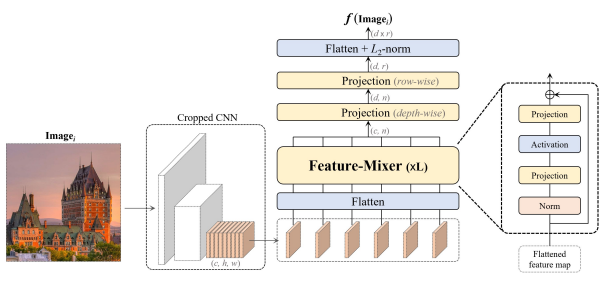
\includegraphics[scale=0.7]{pics/Proposal/mixvpr.png}
    \caption{Tổng quát quá trình xử lý ảnh của MixVPR}
\end{figure}
Với ảnh đầu vào là $I$, mô hình CNN cơ sở sẽ trích xuất ra được tập Feature Map có dạng $F \in R^{c \cdot h \cdot w}$ từ những lớp trung gian.
$$
F = CNN(I)
$$
Ở những phương pháp trước như NetVLAD \cite{arandjelović2016netvlad} và PatchNetVLAD \cite{hausler2021patchnetvlad}, những lớp Feature Map thuộc $F$ sẽ được xem như là một mô tả tương ứng với một miền tiếp nhận trong ảnh ban đầu. Ngược lại, MixVPR xem tensor $F$ như một tập các đặc trưng 2D có kích thước $h \cdot w$.
$$
F = \{X^{i}\}    i = \{1,...c\}
$$
với $X^{i}$ tương ứng với bản đồ kích hoạt thứ $i$ ở F. Ở cách biểu diễn này, mỗi Feature Map không chỉ đại diện cho một miền tiếp nhận trong ảnh mà sẽ chứa một loại thông tin đặc thù cho toàn bộ ảnh. $X^{i}$ sau đó sẽ được định dạng lại thành ma trận một chiều, có được $F \in R^{c \cdot n}$ với $n = h*w$.

Sau đó, dữ liệu sẽ được đưa qua khối Feature Mixer, gồm $L$ những lớp mạng MLP. Những lớp này sẽ nhận vào từng Feature Map $X^{i}$ một chiều và tích hợp thông tin về mối liên kết giữa các giá trị của $X^{i}$ lên chính nó thông qua cách sau:
$$
X^{i} \leftarrow Norm(X^{i})
$$

$$
X^{i} \leftarrow W_2(\sigma(W_1 X^{i}))
$$
với $W_1$ và $W_2$ là trọng số của hai lớp liên kết đầy đủ, cấu tạo nên MLP và $\sigma$ là hàm tạo sự phi tuyến tính cho quá trình xử lý(ReLU). Kỹ thuật nối tắt được sử dụng để nối đầu vào đã qua lớp chuẩn hóa với đầu ra nhằm giúp độ dốc trong quá trình huấn luyện có thể được truyền tải dễ hơn, cải thiện quá trình huấn luyện.

Mục đích của việc sử dụng Feature Mixer là để tận dụng khả năng tổng hợp thông tin từ dữ liệu của các lớp kết nối đầy đủ, thay vì học trên những đặc trưng cục bộ trên ảnh và sử dụng cơ chế tập trung. Ngoài ra, Feature Mixer cũng sẽ trả về kết quả có định dạng như cũ, thay vì có đầu ra giảm dần như những phương pháp tổng hợp dạng phân cấp(kim tự tháp) như trước đây, để mỗi nơ-ron đều có thể biết được thông tin của toàn bộ ảnh. Những lớp MLP trong khối Feature Mixer sẽ giúp tích hợp thông tin trên toàn bộ ảnh qua mỗi lần xử lý.

Mỗi khối Feature Mixer sau khi xử lý xong từng Feature Map trong tập $F \in R^{c \cdot n}$, sẽ ghép kết quả lại, tạo thành $Z \in R^{c \cdot n}$ với cùng kích thước trước khi được đưa vào khối Feature Mixer kế tiếp. Quá trình này có thể được miêu tả bằng công thức sau:
$$
Z = FM_L(FM_{L-1}(\dots FM_1(F)))
$$
Số chiều của $Z$ thường sẽ rất cao do có định dạng được giữ nguyên so với $F$. Để giúp giảm bớt số chiều của $Z$ lại sau khi qua khối Feature Mixer, hai lớp kết nối đầy đủ sẽ được sử dụng để tổng hợp giữa các kênh với nhau và sau đó là giữa các giá trị trong từng kênh. Tác vụ này thực hiện việc tổng hợp có chọn lọc nhằm điều khiển được kích thước của giá trị đầu ra.

Đầu tiên, dữ liệu sẽ được tổng hợp số kênh để biến định dạng của $Z$ từ $R^{c \cdot n}$ thành $R^{d \cdot n}$.
$$
Z' = W_d(Transpose(Z))
$$
với $W_d$ là trọng số của lớp kết nối đầy đủ đầu tiên.

Sau đó, giá trị trên từng kênh sẽ được tổng hợp lại, từ định dạng $R^{d \cdot n}$ thành $R^{d \cdot r}$.
$$
O = W_r(Transpose(Z'))
$$
với $W_r$ là trọng số của lớp kết nối đầy đủ thứ hai.

Kết quả $O$ cuối cùng, có định dạng là $R^{d \cdot r}$, sẽ được ép thành một chiều và chuẩn hóa theo L2 như những phương pháp VPR khác \cite{arandjelović2016netvlad,berton2022rethinking}. Cuối cùng, từ ảnh đầu vào $I$, mô hình sẽ trả về một đoạn mã hóa biểu diễn cho nội dung của ảnh. Đoạn mã hóa này sau đó có thể được dùng để so sánh với đoạn mã hóa của những hình khác nhằm tìm những ảnh tương đồng với $I$.

\subsection{Mô hình tương quan 2D-2D của Map-free Relocalization \cite{arnold2022mapfree}}
\subsubsection*{Ý tưởng đằng sau mô hình}
\subsubsection*{Những bước xử lý của mô hình}

\section{Tiêu chí đánh giá}
\subsection{MixVPR}
\subsection{Mô hình tương quan 2D-2D của Map-free Relocalization}


